\documentclass{beamer}
\mode<presentation>
{
  \usetheme{Warsaw}
  \definecolor{mcgarnet}{rgb}{0.38, 0, 0.08}
  \definecolor{mcgray}{rgb}{0.6, 0.6, 0.6}
  \setbeamercolor{structure}{fg=mcgarnet,bg=mcgray}
  %\setbeamercovered{transparent}
}


\usepackage[english]{babel}
\usepackage[latin1]{inputenc}
\usepackage{times}
\usepackage[T1]{fontenc}
\usepackage{tikz}
\usepackage{graphicx}
\usepackage{animate}

\newcommand{\imagesource}[1]{{\centering\hfill\break\hbox{\scriptsize Image Source:\thinspace{\small\itshape #1}}\par}}

\newcounter{question}

\title{Review and Recursion}


\author{Robert Lowe\\}

\institute[Maryville College] % (optional, but mostly needed)
{
  Division of Mathematics and Computer Science\\
  Maryville College
}

\date[]{}
\subject{}

\pgfdeclareimage[height=0.5cm]{university-logo}{images/Maryville-College}
\logo{\pgfuseimage{university-logo}}



\AtBeginSection[]
{
  \begin{frame}<beamer>{Outline}
    \tableofcontents[currentsection]
  \end{frame}
}


\begin{document}

\begin{frame}
  \titlepage
\end{frame}

\begin{frame}{Outline}
  \tableofcontents
\end{frame}


% Structuring a talk is a difficult task and the following structure
% may not be suitable. Here are some rules that apply for this
% solution: 

% - Exactly two or three sections (other than the summary).
% - At *most* three subsections per section.
% - Talk about 30s to 2min per frame. So there should be between about
%   15 and 30 frames, all told.

% - A conference audience is likely to know very little of what you
%   are going to talk about. So *simplify*!
% - In a 20min talk, getting the main ideas across is hard
%   enough. Leave out details, even if it means being less precise than
%   you think necessary.
% - If you omit details that are vital to the proof/implementation,
%   just say so once. Everybody will be happy with that.

\section{Midterm Exam Review}
\begin{frame}
    \frametitle{Questions 1-10}
    \begin{enumerate}[<+->]
        \item What are some of the main challenges in modern software development?
        \item What is object oriented programming?
        \item How do parts of speech represented in object oriented programming?
        \item What are the four major principles of object oriented programming?
        \item What are the main goals of object oriented programming?
        \item Know the syntax for class declaration.
        \item Be able to write a class implementation.
        \item What is the purpose of constructors?
        \item In best OOP practice, what is the minimal set of constructors that you need to provide with all classes?
        \item What is a destructor and when should you provide one?
        \setcounter{question}{\value{enumi}}
    \end{enumerate}
\end{frame}

\begin{frame}
    \frametitle{Questions 11-22}
    \begin{enumerate}[<+->]
        \setcounter{enumi}{\value{question}}
        \item What is a pointer?  What value does a pointer store?
        \item How do you declare a pointer?
        \item How can you retrieve the address of a variable?
        \item How do you dereference a pointer? 
        \item What does dereferencing a pointer do?
        \item Be able to write pointer based code.
        \item How do you dynamically allocate objects?
        \item How do you destroy dynamically allocated objects?
        \item What is a memory leak, and how can they be avoided?
        \item How do you access methods and attributes of an object using a pointer to the object?
        \item What are the advantages of using pointers with objects?
        \item What are terminal control codes?
        \setcounter{question}{\value{enumi}}
    \end{enumerate}
\end{frame}

\begin{frame}
    \frametitle{Questions 23-32}
    \begin{enumerate}[<+->]
        \setcounter{enumi}{\value{question}}
        \item What is meant by an "is-a" relationship?  Be able to provide some examples!
        \item What is class inheritance?
        \item What is meant by public inheritance?  How about private inheritance?
        \item What is function overriding, and how does it work?
        \item What is polymorphism?
        \item What are virtual functions, and how do they relate to polymorphism?
        \item Can constructors be virtual?
        \item Can destructors be virtual?
        \item What is the best practice regarding virtual functions?
        \item What are pure virtual functions, and why are they important?
        \setcounter{question}{\value{enumi}}
    \end{enumerate}
\end{frame}

\begin{frame}
    \frametitle{Questions 33-43}
    \begin{enumerate}[<+->]
        \setcounter{enumi}{\value{question}}
        \item What is meant by up-casting and down-casting?
        \item What are overloaded operators?
        \item Know the syntax for creating an overloaded operator as a stand-alone function.
        \item Know the syntax for creating an overloaded operator as a member of a class.
        \item What are the best practices for using overloaded operators?
        \item What is meant by "software engineering"?
        \item What is the waterfall method?
        \item What is meant by "agile methods"?
        \item Know how to construct and use the following UML diagrams: Use Case, Object, Sequence, and Class.
        \item What is Object Oriented Analysis and Design?  Be able to carry it out on a sample problem.
        \item Know how the UML diagrams fit into the OOAD process.
        \setcounter{question}{\value{enumi}}
    \end{enumerate}
\end{frame}

\section{Better Living Through Recursion}
\begin{frame}
    \frametitle{To understand recursion...}
    \begin{columns}
        \column{0.5\textwidth}
        Recursion is...
        \begin{itemize}[<+->]
            \item When a function re-enters itself.
            \item Used when a problem is solved by 
                solving smaller versions of itself.
            \item Solves many interesting and complex
                problems.
        \end{itemize}
        \column{0.5\textwidth}
        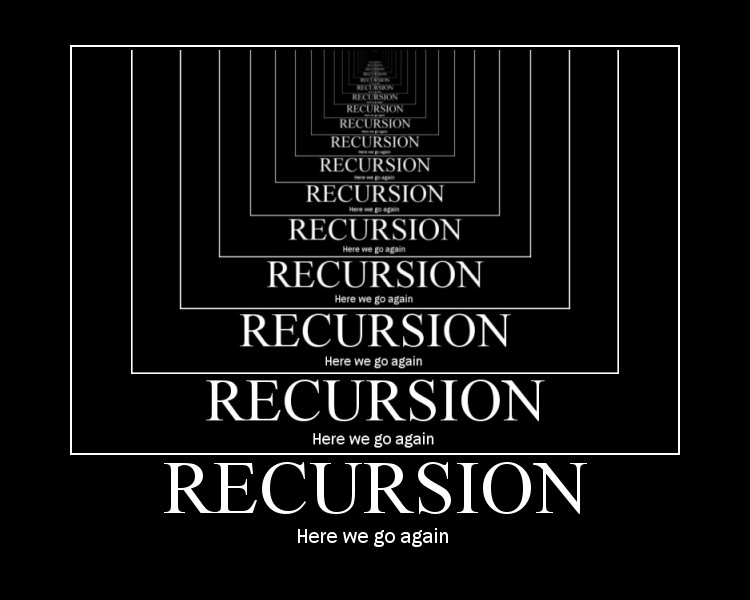
\includegraphics[width=\textwidth]{images/recursion}
        \imagesource{https://prateekvjoshi.com/}
    \end{columns}
\end{frame}

\begin{frame}
    \frametitle{... you must first understand recursion.}
    Ingredients of Recrusion:
    \begin{description}[<+->]
    \item[Base Case] The condition where recursion stops.
    \item[Recursive Case] The condition where we make a 
        recursive call to form the complete solution.
    \end{description}
    
    \begin{block}{Recursion Syntax}<+->
        There is no special syntax for recursion in C++!
        It's just a programming technique!
    \end{block}
    
    \begin{block}{Once you Understand Recursion}
        You will understand recursion.
    \end{block}
\end{frame}

\begin{frame}
    \frametitle{Recursive Problems}
    \begin{columns}
    \column{0.5\textwidth}
        \begin{itemize}[<+->]
            \item Divide and Conquer Algorithms
            \item Mathematical Recurrence Relations
            \item Recursive Data Structures
            \item Language Processing
            \item Artificial Intelligence
            \item Fractals (example: Koch Curve)
            \item Searching Candidate Solutions
        \end{itemize}
    \column{0.5\textwidth}
        \begin{overprint}
        \onslide<1>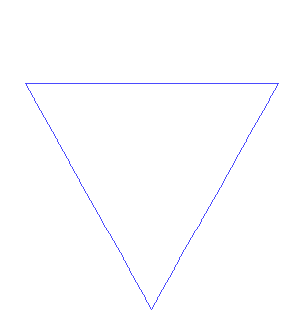
\includegraphics[width=\textwidth]{images/koch-0}
        \onslide<2>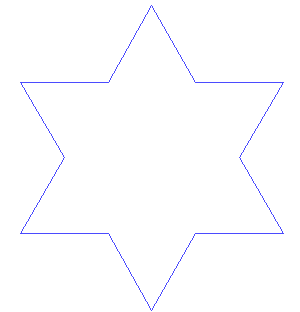
\includegraphics[width=\textwidth]{images/koch-1}
        \onslide<3>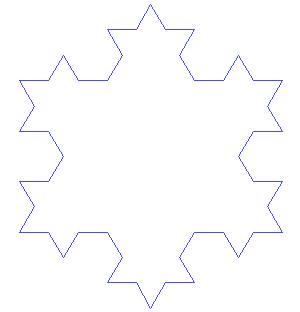
\includegraphics[width=\textwidth]{images/koch-2}
        \onslide<4>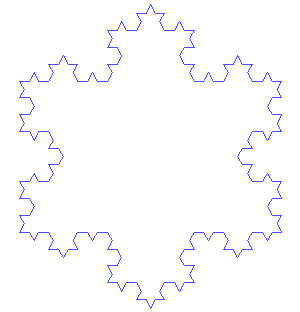
\includegraphics[width=\textwidth]{images/koch-3}
        \onslide<5>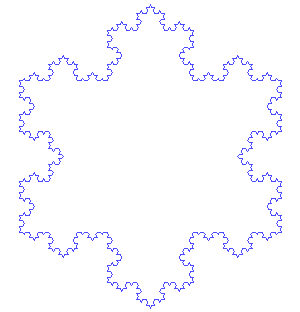
\includegraphics[width=\textwidth]{images/koch-4}
        \onslide<6>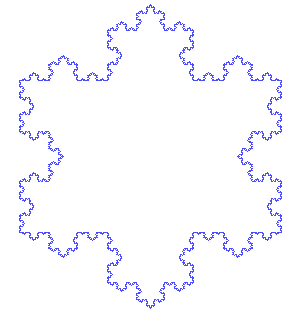
\includegraphics[width=\textwidth]{images/koch-5}
        \onslide<7->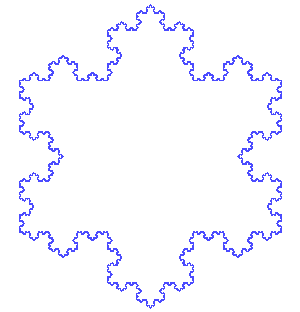
\includegraphics[width=\textwidth]{images/koch-6}
        \end{overprint}
        \imagesource{wikipedia.org}
    \end{columns}
\end{frame}

\begin{frame}[fragile]
    \frametitle{Example: Greatest Common Denominator}
    \[
    \gcd(x,y) =
    \begin{cases}
         x & \mbox{if } y = 0 \\
         \gcd(y, \operatorname{remainder}(x,y)) & \mbox{if } y > 0 \\
     \end{cases}
     \]
     \defverbatim{\gcdImplementation}{%
         \begin{verbatim}
int gcd(int x, int y)
{
    if(y == 0) {
        return x;
    }
    
    return gcd(y, x%y);
}
         \end{verbatim}
      }
      \only<+->{\gcdImplementation}
\end{frame}


\end{document}